%!TEX program = xelatex

% \documentclass[10pt]{article}
%%%%%%%%%%%%%%%%%%%%%%%%%%%%%%%%%%%%%%%%%
% Modified By Orcuslc, 2016-9-12
% http://github.com/orcuslc
%
% Wilson Resume/CV
% Structure Specification File
% Version 1.0 (22/1/2015)
%
% This file has been downloaded from:
% http://www.LaTeXTemplates.com
%
% License:
% CC BY-NC-SA 3.0 (http://creativecommons.org/licenses/by-nc-sa/3.0/)
%
%%%%%%%%%%%%%%%%%%%%%%%%%%%%%%%%%%%%%%%%%

%----------------------------------------------------------------------------------------
%	PACKAGES AND OTHER DOCUMENT CONFIGURATIONS
%----------------------------------------------------------------------------------------

\usepackage[a4paper, hmargin=25mm, vmargin=30mm, top=20mm]{geometry} % Use A4 paper and set margins

\usepackage{fancyhdr} % Customize the header and footer

\usepackage{lastpage} % Required for calculating the number of pages in the document

\usepackage{hyperref} % Colors for links, text and headings

\setcounter{secnumdepth}{0} % Suppress section numbering

%\usepackage[proportional,scaled=1.064]{erewhon} % Use the Erewhon font
%\usepackage[erewhon,vvarbb,bigdelims]{newtxmath} % Use the Erewhon font
\usepackage[utf8]{inputenc} % Required for inputting international characters
\usepackage[T1]{fontenc} % Output font encoding for international characters

\usepackage{fontspec} % Required for specification of custom fonts
\setmainfont[Path = ./fonts/,
Extension = .otf,
BoldFont = Erewhon-Bold,
ItalicFont = Erewhon-Italic,
BoldItalicFont = Erewhon-BoldItalic,
SmallCapsFeatures = {Letters = SmallCaps}
]{Erewhon-Regular}

\usepackage{color} % Required for custom colors
\definecolor{slateblue}{rgb}{0.17,0.22,0.34}

\usepackage{sectsty} % Allows customization of titles
\sectionfont{\color{slateblue}} % Color section titles

\fancypagestyle{plain}{\fancyhf{}\cfoot{\thepage\ of \pageref{LastPage}}} % Define a custom page style
\pagestyle{plain} % Use the custom page style through the document
\renewcommand{\headrulewidth}{0pt} % Disable the default header rule
\renewcommand{\footrulewidth}{0pt} % Disable the default footer rule

\setlength\parindent{0pt} % Stop paragraph indentation

% Non-indenting itemize
\newenvironment{itemize-noindent}
{\setlength{\leftmargini}{0em}\begin{itemize}}
{\end{itemize}}

% Text width for tabbing environments
\newlength{\smallertextwidth}
\setlength{\smallertextwidth}{\textwidth}
\addtolength{\smallertextwidth}{-2cm}

\newcommand{\sqbullet}{~\vrule height 1ex width .8ex depth -.2ex} % Custom square bullet point definition

%----------------------------------------------------------------------------------------
%	MAIN HEADER COMMAND
%----------------------------------------------------------------------------------------

\renewcommand{\title}[1]{
{\huge{\color{slateblue}\textbf{#1}}}\\ % Header section name and color
\rule{\textwidth}{0.5mm}\\ % Rule under the header
}

%----------------------------------------------------------------------------------------
%	JOB COMMAND: Modified by Orcuslc 2016-09-12
%----------------------------------------------------------------------------------------

\newcommand{\job}[6]{
\begin{tabbing}
\hspace{2cm} \= \kill
\textbf{#1} \> \href{#4}{\textbf{#3}} \\
\textbf{#2} \>\+ \textit{#5} \\
\begin{minipage}{\smallertextwidth}
\vspace{2mm}
#6
\end{minipage}
\end{tabbing}
\vspace{2mm}
}

%----------------------------------------------------------------------------------------
%	SKILL GROUP COMMAND - Modified by Orcuslc 2016-09-12
%----------------------------------------------------------------------------------------

\newcommand{\skillgroup}[2]{
% \begin{tabbing}
% \hspace{5mm} \= \kill
% \sqbullet \> \textbf{#1}
% \end{tabbing}
% \begin{tabbing}
% \vspace{-2pt}
% \hspace{3cm} \= \kill
% #2
% \end{tabbing}
% }
\begin{tabbing}
\hspace{5mm} \= \kill
\sqbullet \>\+ \textbf{#1} \\

\begin{minipage}{\smallertextwidth}
\vspace{2mm}
#2
\end{minipage}
\end{tabbing}
}

\newcommand{\skill}[2]{
\begin{tabbing}
\hspace{1cm} \> \hspace{3cm} \= \kill
\>\textbf{#1:} \> #2 \\
\end{tabbing}
% \hspace
}

%----------------------------------------------------------------------------------------
%	INTERESTS GROUP COMMAND
%-----------------------------------------------------------------------------------------

\newcommand{\interestsgroup}[1]{
\begin{tabbing}
\hspace{5mm} \= \kill
#1
\end{tabbing}
\vspace{-10mm}
}

\newcommand{\interest}[1]{\sqbullet \> \textbf{#1}\\[3pt]} % Define a custom command for individual interests


%---------------------------------------------------------------
%   AWARDS GROUP COMMAND: Created by Orcuslc 2016-09-12
%---------------------------------------------------------------
\newcommand{\awardgroup}[1]{
\begin{tabbing}
\hspace{5mm} \= \kill
#1
\end{tabbing}
\vspace{2mm}
}

\newcommand{\award}[2]{
% \begin{tabbing}
% \hspace{0} \> \hspace{2cm} \= \kill
\hspace{2cm} \> \hspace{2cm} \= \kill
\sqbullet \> \textbf{#1} \> #2 \\[3pt]
% \hspace{2cm} \= \kill
% \end{tabbing}

}

%----------------------------------------------------------------------------------------
%	TABBED BLOCK COMMAND: Modified by Orcuslc 2016-09-12
%----------------------------------------------------------------------------------------

\newcommand{\tabbedblock}[1]{
\begin{tabbing}
\hspace{2cm} \= \hspace{4cm} \= \hspace{4cm} \= \hspace{4cm} \= \kill
#1
\end{tabbing}
}

%-----------------------------------------------------------------
%  TABBED BLOCK 2 COMMAND: Created by Orcuslc 2016-09-12
%-----------------------------------------------------------------
\newcommand{\tabblock}[5]{
\begin{tabbing}
% \hspace{2cm} \= \kill
\hspace{2cm} \= \hspace{4cm} \= \hspace{4cm} \= \hspace{4cm} \= \kill

\textbf{#1} \> \textbf{#3} \\
\textbf{#2} \> \textbf{#4} \\[5pt]
\>\+
#5
\end{tabbing}
}


%-----------------------------------------------------------------
%  RESEARCH COMMAND: Created by Orcuslc 2016-09-12
%-----------------------------------------------------------------
\newcommand{\research}[7]{
\begin{tabbing}
\hspace{2cm} \= \kill
\textbf{#1} \> \textbf{#3}, under the supervision of \href{#5}{\textbf{#4}} \\
% \href{#4}{#3} \\
\textbf{#2} \>\+ \textit{#6} \\
\begin{minipage}{\smallertextwidth}
\vspace{0.5mm}
#7
\end{minipage}
\end{tabbing}
\vspace{2mm}
}

%-------------------------------------------------------------------------
%      Programming Projects Command - Created by Orcuslc 2016-9-14
%-------------------------------------------------------------------------
% \newcommand{\projectgroup}[1]{
% \begin{tabbing}
% % \hspace{5mm} \= \kill
% \vspace{5mm}
% #1
% \end{tabbing}
% }

\newcommand{\projectgroup}[1]{
% \begin{tabbing}
\hspace{5mm} \= \kill
#1
% \end{tabbing}
\vspace{2mm}
}


\newcommand{\project}[3]{
% \begin{tabbing}
\hspace{2cm} \> \hspace{2cm} \= \kill
\sqbullet \> \textbf{#1} \> #2 \\
\> \textbf{code:} \> \href{#3}{#3} \\[5pt]
% \end{tabbing}
}
\usepackage{epstopdf}
\usepackage{graphics}
\usepackage{subfig}
\usepackage{listings}
\lstset{
  numbers=left,
    framexleftmargin=10mm,
    frame=none,
    backgroundcolor=\color[RGB]{245,245,244},
  keywordstyle=\bf\color{blue},
  identifierstyle=\bf,
  numberstyle=\color[RGB]{0,192,192},
  commentstyle=\it\color[RGB]{0,96,96},
  stringstyle=\rmfamily\slshape\color[RGB]{128,0,0},
  showstringspaces=false,
  extendedchars=false
    }
\DeclareGraphicsExtensions{.eps,.ps,.jpg,.bmp}

\begin{document}

\title{Homework 2}{16.10.9}

% \parbox{0.3\textwidth}{
% Chuan Lu}
% \hfill
% \parbox{0.3\textwidth}{
% 13300180056}
% \hfill
% \parbox{0.3\textwidth}{
% chuanlu13@fudan.edu.cn}

\problem{1}{Explain the relationship between spectral clustering, normalized spectral clustering and graph cut.}
\solution{Solution}{
We assume $k=2$ in the following explanation. \n
For spectral clustering, we already know that the eigenvector $u_2$ corresponding to the second smallest eigenvalue $\lambda_2$ of the Laplacian matrix of the graph is the solution for the minimization
$$ \min_{\tbf{f}} \ \tbf{f}^\top\tbf{L}\tbf{f},$$
$$s.t. \quad \tbf{f}^\top \tbf{f} = 1, \tbf{f}^\top\tbf{1} = 0$$
In fact, if we define 
$$G(f) = G(f_1,\cdots, f_n) = f\tr\tbf{L}f - \lambda_1 (f\tr f-1) - \lambda_2 f\tr\tbf{1} $$ $$ =  \frac{1}{2}\sum_{i,j=1}^{n}w_{ij}(f_i-f_j)^2-\lambda_1(\sum_{i=1}^{n}f_i^2-1)-\lambda_2\sum_{i=1}^n f_i$$
Then according to Lagrange Theorm, we let
$$\frac{\partial G}{\partial f_i} = \sum_{j=1}^n (f_i-f_j) - 2\lambda_1 f_i - \lambda_2 = 0, \quad  i=1:n$$
If we add the $n$ equations, we get
$$2\lambda_1\sum_{i, j=1}^n f_i + n\lambda_2=0$$
Since $f\tr\tbf{1} = 0$, then $\lambda_2 = 0$. So
$$\sum_{j=1}^n w_{ij}f_{j} = \lambda f_i,\quad \lambda = \sum_{j=1}^{n}w_{ij}-2\lambda_1,\quad i=1:n, $$
which means $f$ is an eigenvector of $\tbf{L}$.\n
For Min Cut, if we define $\tbf{f} = (f_1, f_2\cdots f_n)^\top\in\mbb{R}^n$,
$$\bra{f_i}{1}{-1}{if\ v_i\in\mbb{A}}{if\ v_i\in\mbb{\bar{A}}}$$
Then
$$\bra{(f_i-f_j)^2}{4}{0}{i\in\mbb{A},j\in\mbb{\bar{A}}}{else}$$
So 
$$MCut(A_1,\cdots,A_k) = \sum_{i=1}^{k}cut(A_i, \bar{A_i}) = \frac{1}{4}f\tr\tbf{L}f$$
We can minimize this with the $f$ from spectral clustering. \n
For Ratio Cut, we can define $f$ as
$$\bra{f_i}{\sqrt{\vt{\bar{A}}/\vt{\bar{A}}}}{-\sqrt{\vt{A}/\vt{\bar{A}}}}{v_i\in\mbb{A}}{v_i\in\mbb{\bar{A}}}$$
Then
$$\bra{(f_i-f_j)^2}{\frac{\vt{A}}{\vt{\bar{A}}}+\frac{\vt{\bar{A}}}{\vt{A}}+2}{0}{v_i, v_j\ in \ the \ same \ part}{else}$$
So 
$$RCut(A, \bar{A}) = \frac{1}{2}\frac{\vt{A}\vt{\bar{A}}}{(\vt{A}+\vt{\bar{A}})^2}\frac{1}{\vt{A}+\vt{\bar{A}}}\sum_{i, j}(f_i-f_j)^2w_{ij}=\frac{f\tr\tbf{L}f}{2n^2}$$
For normalized spectral clustering, we have
$$L_{sym} = I - D^{-1/2}WD^{-1/2} = D^{-1/2}LD^{-1/2}$$
and normalized cut can be done using $g^*$, the Fiedler vector of $D^{-1/2}LD^{-1/2}.$ \\[1cm]
When $k \geq 3$, we can find $k$ points $x_i$ in $\mbb{R}^k$, s.t. $\vt{x_i-x_j} = \vt{x_k - x_l}$, for each $i, j, k, l$. \\
Then define $f_i = x_i$, and it is same with $k = 2$.
}

\problem{2}{Cluster Data.csv with spectral clustering, construct three different graphs and compare the difference with result of K-means.}
\solution{Solution}{
For Data1.csv, the result is shown as follows.
\begin{figure}[htbp]
\centering
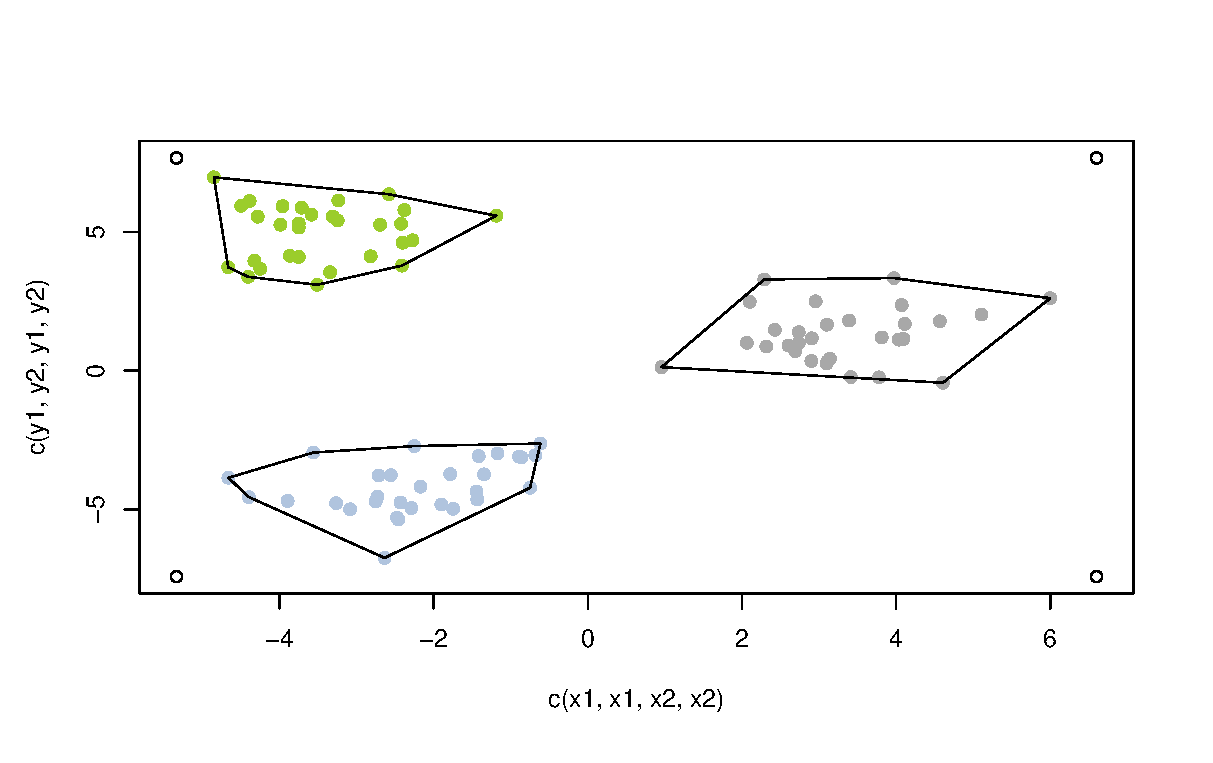
\includegraphics[width = 10cm]{pics/hw2_2_data1_kmeans.eps}
\caption{Kmeans}
\label{Kmeans for data 1}
\end{figure}
\begin{figure}[htbp]
\centering
\subfloat[Full-connect1]{ %
	\includegraphics[width = 0.45\textwidth]{pics/hw2_2_data1_full_1.eps}}\hfill
\subfloat[Full-connect2]{
	\includegraphics[width = 0.45\textwidth]{pics/hw2_2_data1_full_2.eps}}
\end{figure}
\begin{figure}[htbp]
\centering
\subfloat[Epsilon = 0.1]{ %
	\includegraphics[width = 0.3\textwidth]{pics/hw2_2_data1_epsilon_01.eps}}\hfill
\subfloat[Epsilon = 1]{
	\includegraphics[width = 0.3\textwidth]{pics/hw2_2_data1_epsilon_1.eps}}\hfill
\subfloat[Epsilon = 3]{
	\includegraphics[width = 0.3\textwidth]{pics/hw2_2_data1_epsilon_3.eps}}	
\end{figure}
\begin{figure}[htbp]
\centering
\subfloat[Directed, n = 3]{ %
	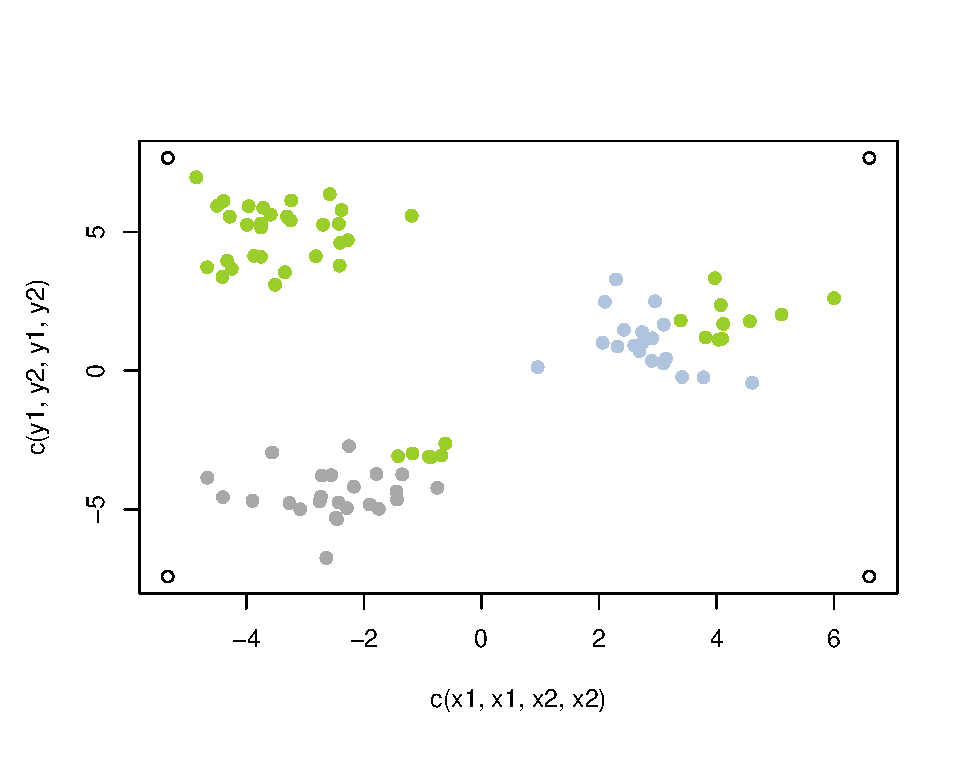
\includegraphics[width = 0.3\textwidth]{pics/hw2_2_data1_directed_3.eps}}\hfill
\subfloat[Directed, n = 5]{
	\includegraphics[width = 0.3\textwidth]{pics/hw2_2_data1_directed_5.eps}}\hfill
\subfloat[Directed, n = 10]{
	\includegraphics[width = 0.3\textwidth]{pics/hw2_2_data1_directed_10.eps}}	
\end{figure}
\begin{figure}[htbp]
\centering
\subfloat[Undirected, n = 3]{ %
	\includegraphics[width = 0.3\textwidth]{pics/hw2_2_data1_undirected_3.eps}}\hfill
\subfloat[Undirected, n = 5]{
	\includegraphics[width = 0.3\textwidth]{pics/hw2_2_data1_undirected_5.eps}}\hfill
\subfloat[Undirected, n = 20]{
	\includegraphics[width = 0.3\textwidth]{pics/hw2_2_data1_undirected_20.eps}}	
\end{figure}
\\[1cm]
For Data3.csv, the result is shown as follows.
\begin{figure}[htbp]
\centering
\includegraphics[width = 10cm]{pics/hw2_2_data3_kmeans.eps}
\caption{Kmeans}
\label{Kmeans for data 3}
\end{figure}
\begin{figure}[htbp]
\centering
\subfloat[Full-connect1]{ %
	\includegraphics[width = 0.45\textwidth]{pics/hw2_2_data3_full_1.eps}}\hfill
\subfloat[Full-connect2]{
	\includegraphics[width = 0.45\textwidth]{pics/hw2_2_data3_full_2.eps}}
\end{figure}
\begin{figure}[htbp]
\centering
\subfloat[Epsilon = 0.1]{ %
	\includegraphics[width = 0.3\textwidth]{pics/hw2_2_data3_epsilon_0_1.eps}}\hfill
\subfloat[Epsilon = 2]{
	\includegraphics[width = 0.3\textwidth]{pics/hw2_2_data3_epsilon_2.eps}}\hfill
\subfloat[Epsilon = 5]{
	\includegraphics[width = 0.3\textwidth]{pics/hw2_2_data3_epsilon_5.eps}}	
\end{figure}
\begin{figure}[htbp]
\centering
\includegraphics[width = 10cm]{pics/hw2_2_data3_directed_3.eps}
\caption{directed, n = 3}
\end{figure}
\begin{figure}[htbp]
\centering
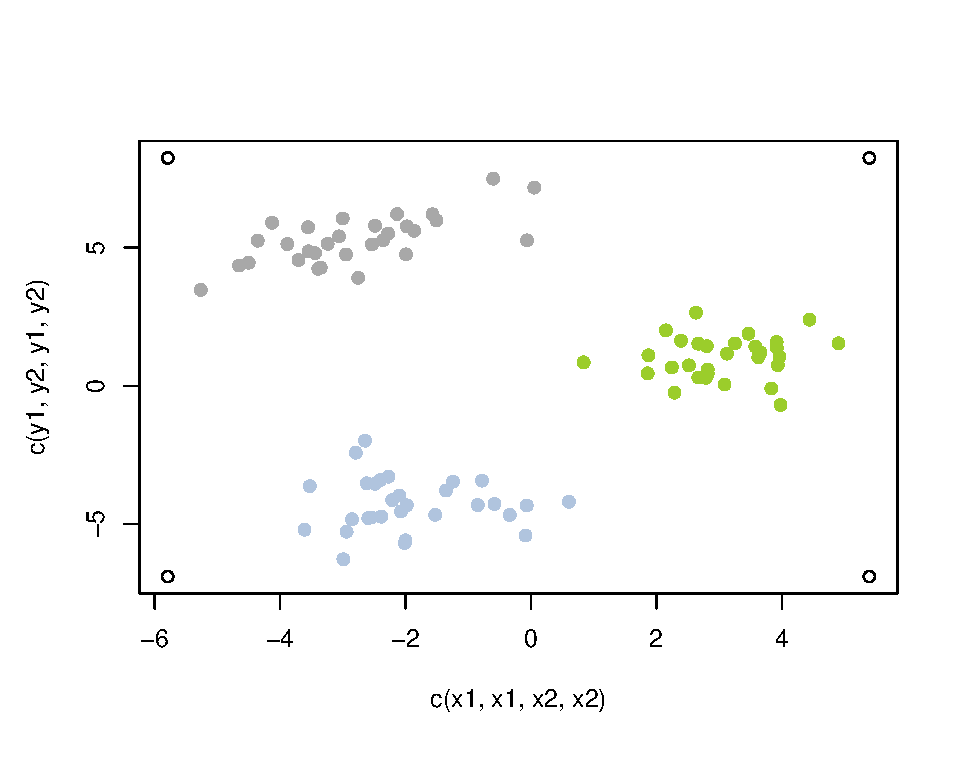
\includegraphics[width = 10cm]{pics/hw2_2_data3_undirected_3.eps}
\caption{Undirected, n = 3}
\end{figure} \\
From the results we can know that for these groups, spectral clustering is not always better than kmeans. The parameters in spectral clustering are also important.
}
\newpage

\problem{3}{Cluster circles, curves with spectral clustering}
\solution{Solution}{
The results of circles.csv is as follows.
\begin{figure}[htbp]
\centering
\includegraphics[width = 10cm]{pics/hw2_3_circle_full.eps}
\caption{full connection}
\end{figure}
\begin{figure}[htbp]
\centering
\subfloat[epsilon = 1]{ %
	\includegraphics[width = 0.45\textwidth]{pics/hw2_3_circle_epsilon_1.eps}}\hfill
\subfloat[epsilon = 2]{
	\includegraphics[width = 0.45\textwidth]{pics/hw2_3_circle_epsilon_2.eps}}
\end{figure}
\begin{figure}[htbp]
\centering
\subfloat[directed, n = 5]{ %
	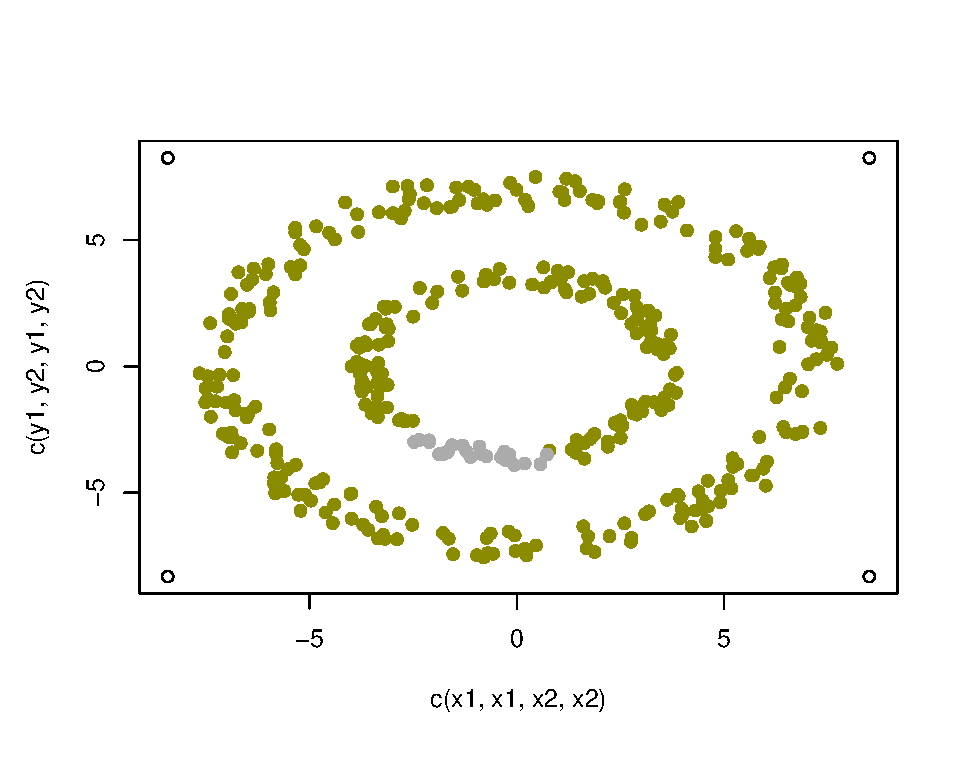
\includegraphics[width = 0.45\textwidth]{pics/hw2_3_circle_directed_5.eps}}\hfill
\subfloat[directed, n = 10]{
	\includegraphics[width = 0.45\textwidth]{pics/hw2_3_circle_directed_10.eps}}
\end{figure}
\begin{figure}[htbp]
\centering
\subfloat[undirected, n = 2]{ %
	\includegraphics[width = 0.45\textwidth]{pics/hw2_3_circle_undirected_2.eps}}\hfill
\subfloat[undirected, n = 5]{
	\includegraphics[width = 0.45\textwidth]{pics/hw2_3_circle_undirected_5.eps}}
\end{figure}
\\
The result of curves.csv is shown as follows.
\begin{figure}[htbp]
\centering
\includegraphics[width = 10cm]{pics/hw2_3_curve_full.eps}
\caption{full connection}
\end{figure}
\begin{figure}[htbp]
\centering
\subfloat[epsilon = 1]{ %
	\includegraphics[width = 0.3\textwidth]{pics/hw2_3_curve_epsilon_1.eps}}\hfill
\subfloat[epsilon = 3]{
	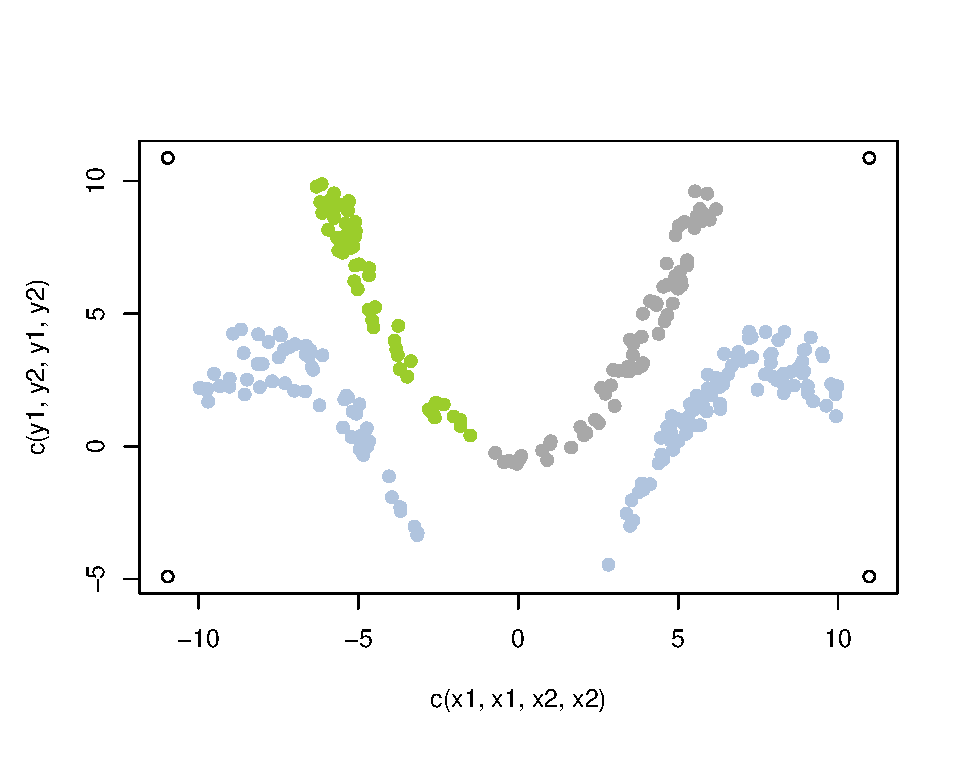
\includegraphics[width = 0.3\textwidth]{pics/hw2_3_curve_epsilon_3.eps}}\hfill
\subfloat[epsilon = 10]{
	\includegraphics[width = 0.3\textwidth]{pics/hw2_3_curve_epsilon_10.eps}}
\end{figure}
\begin{figure}[htbp]
\centering
\subfloat[directed, n = 10]{ %
	\includegraphics[width = 0.3\textwidth]{pics/hw2_3_curve_directed_10.eps}}\hfill
\subfloat[directed, n = 20]{
	\includegraphics[width = 0.3\textwidth]{pics/hw2_3_curve_directed_20.eps}}\hfill
\subfloat[directed, n = 30]{
	\includegraphics[width = 0.3\textwidth]{pics/hw2_3_curve_directed_30.eps}}
\end{figure}
\begin{figure}[htbp]
\centering
\subfloat[undirected, n = 5]{ %
	\includegraphics[width = 0.45\textwidth]{pics/hw2_3_curve_undirected_5.eps}}\hfill
\subfloat[undirected, n = 10]{
	\includegraphics[width = 0.45\textwidth]{pics/hw2_3_curve_undirected_10.eps}}
\end{figure}
}












% \begin{figure}[htbp]
% \centering
% \includegraphics[width = 10cm]{pics/hw2_data1_cluster.eps}
% \caption{The clusters of Data1.csv with k = 3}
% \label{clusters of data1}
% \end{figure}
% \\[1mm]
% \problem{2}{Cluster $Data_i.csv$ with K-means, judge the number of clusters, and compare differences between different evaluating methodss.}
% \solution{Solution}{
% The code of K-means, evaluating and test scripts can be found from attachments(kmeans.R, evaluate.R, hw1.2.R).
% }
% \solution{Result}{
% For Data1.csv, we cluster with k = 3. The result is shown as below.
% \begin{figure}[htbp]
% \centering
% \includegraphics[width = 10cm]{pics/hw2_data1_cluster.eps}
% \caption{The clusters of Data1.csv with k = 3}
% \label{clusters of data1}
% \end{figure}
% \\[1mm]

% For choosing k, the result of Data1.csv is shown below; The first is the result of Calinski-Harabasz method, the second Hartigan method and the last Gap Statistic. \\[3pt]
% The result of CH method is 9, if we may add a limit that $k\le 10.$ The result of H method is 3, and result of GAP statistic is 3.\\[3pt]

% \begin{figure}[htbp]
% \centering
% \subfloat[CH method]{ %
% 	\includegraphics[width = 0.3\textwidth]{pics/hw2_data1_k_CH.eps}}\hfill
% \subfloat[H method]{ %
% 	\includegraphics[width = 0.3\textwidth]{pics/hw2_data1_k_H.eps}}\hfill
% \subfloat[GAP statistic]{ %
% 	\includegraphics[width = 0.3\textwidth]{pics/hw2_data1_k_GAP.eps}}\hfill
% \caption{The three evaluating methods of choosing k for Data1.csv}
% \label{EVA Data1}
% \end{figure}

% For Data2.csv, since each data point is of 3 dims, we cannot plot its clustering result here. But after deploying the evaluating methods we consider k = 3. The type of datas can be find in attachments(CLUSTER\_DATA2.txt). \\[3pt]

% The result of CH method is 8, if we limit that $k\le 10$. The result of H method and result of GAP statistic are 3. \\[3pt]
% The pics are shown below.

% \begin{figure}[htbp]
% \centering
% \subfloat[CH method]{ %
% 	\includegraphics[width = 0.3\textwidth]{pics/hw2_data2_k_CH.eps}}\hfill
% \subfloat[H method]{ %
% 	\includegraphics[width = 0.3\textwidth]{pics/hw2_data2_k_H.eps}}\hfill
% \subfloat[GAP statistic]{ %
% 	\includegraphics[width = 0.3\textwidth]{pics/hw2_data2_k_GAP.eps}}\hfill
% \caption{The three evaluating methods of choosing k for Data2.csv}
% \label{EVA Data2}
% \end{figure}

% For Data3.csv, we fix k = 3 after evaluating k with H method and GAP statistic; The result of clustering can be found in attachments(CLUSTER\_DATA3.txt). \\[3pt]

% The result of CH method is 9, if we limit that $k\le 10$. The result of H method and result of GAP statistic are 3. \\[3pt]
% The pics are shown below.

% \begin{figure}[htbp]
% \centering
% \subfloat[CH method]{ %
% 	\includegraphics[width = 0.3\textwidth]{pics/hw2_data3_k_CH.eps}}\hfill
% \subfloat[H method]{ %
% 	\includegraphics[width = 0.3\textwidth]{pics/hw2_data3_k_H.eps}}\hfill
% \subfloat[GAP statistic]{ %
% 	\includegraphics[width = 0.3\textwidth]{pics/hw2_data3_k_GAP.eps}}\hfill
% \caption{The three evaluating methods of choosing k for Data3.csv}
% \label{EVA Data2}
% \end{figure}

% For Data4.csv, we found k = 3 after evaluating k with H method and GAP statistic; The result of clustering can be found in attachments(CLUSTER\_DATA4.txt). \\[3pt]

% The result of CH method is 7, if we limit that $k\le 10$. The result of H method and result of GAP statistic are 3. \\[3pt]
% The pics are shown below.

% \begin{figure}[htbp]
% \centering
% \subfloat[CH method]{ %
% 	\includegraphics[width = 0.3\textwidth]{pics/hw2_data4_k_CH.eps}}\hfill
% \subfloat[H method]{ %
% 	\includegraphics[width = 0.3\textwidth]{pics/hw2_data4_k_H.eps}}\hfill
% \subfloat[GAP statistic]{ %
% 	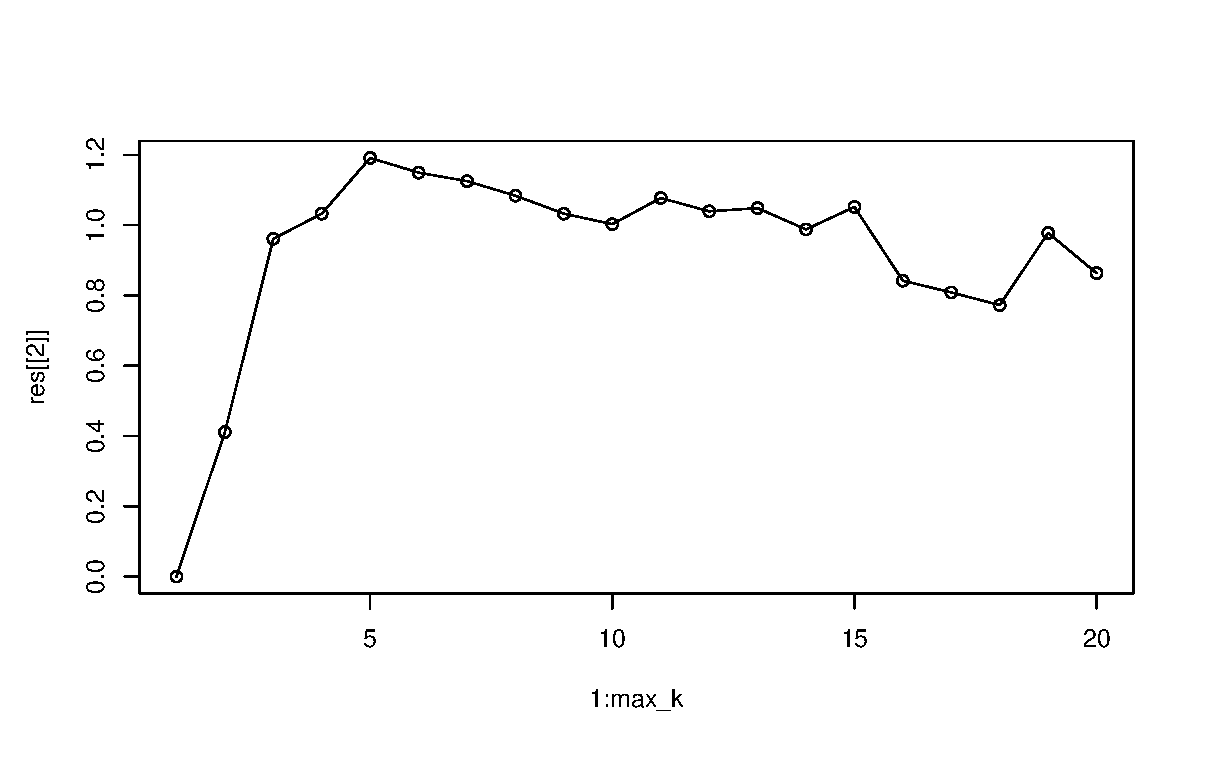
\includegraphics[width = 0.3\textwidth]{pics/hw2_data4_k_GAP.eps}}\hfill
% \caption{The three evaluating methods of choosing k for Data4.csv}
% \label{EVA Data2}
% \end{figure}
% }
% \solution{Analysis}{
% It is suprising that result of Calinski-Harabasz method does not agree with the other methods. I consider it as the result that I misunderstood the meaning of $W(k), B(k)$. I calculate the former as the target function of cluster; the latter as $\sum_{c_i, c_j \in C}\lVert c_i - c_j \rVert^2$, in which $C$ is the set of cluster centers.
% }

% \problem{3}{Use hierarchical clustering methods to cluster $Data_i.csv$}
% \solution{Solution}{
% The code of hierarchical clustering and the test script can be found from attachments(hierarchical\_clustering.R, hw1.3.R).
% }
% \solution{Result}{
% It is somehow embarrassing that I still did't know how to draw trees in R without $hcluster()$. The result can be shown is the attachments, (HC\_DATA1.txt and HC\_DATA2.txt). \\[3pt]
% Each result is a (n-1) * narg matrix, in which n is the number of data points and narg is the number of dims in each data point. Each row in the matrix(for example, A[1, ]) means a step when two points merged with each other; A[1, 1] and A[1, 2] merged into a new A[1, 1], and the point represented by A[1, 2] is abandoned. \\[3pt]
% It is possible to draw the tree and do Tree-Cut with the results.
% }

% \refgroup{
% \reference{a a a a  a a}
% \reference{b b b b b b}
% \reference{c c c c c c}
% \reference{b}

% }


\end{document}